\documentclass[runningheads]{llncs}
\usepackage[T1]{fontenc}
\usepackage{graphicx}
\usepackage{subcaption}
\usepackage[UTF8]{ctex}
\usepackage{enumitem}
\usepackage{tabularx}
\usepackage{booktabs}
\usepackage{multirow}

\bibliographystyle{splncs04}

\AtBeginDocument{%
  \providecommand\BibTeX{{%
    Bib\TeX}}}

\begin{document}

\title{触觉反馈在沉浸式手势学习环境中对物理学习效果的影响研究}

\author{匿名作者}

\maketitle

\begin{abstract}
  随着手势追踪技术的发展,基于虚拟现实(VR)的手势交互环境为物理实验教学提供了直观操作体验,但传统虚拟场景缺乏触觉反馈,导致学生难以建立 “手势操作 - 物理感知” 的关联,制约学习沉浸感与知识理解深度。本研究聚焦沉浸式手势学习环境中触觉反馈对物理学习效果的影响,以高中物理实验为场景设计实证研究。采用多模态数据分析方法,整合物理知识测试、主观问卷量表和客观生理指标,系统探究触觉反馈对交互体验与知识掌握的差异化影响。结果显示:融入触觉反馈的手势交互能(1)显著改善学习者的交互体验,具体表现为学习动机(p<0.001)和沉浸感(p<0.001)显著增强,且未显著增加认知负荷(p=0.602);(2)未达到提升学习者知识掌握水平(p=0.087)的统计显著,但呈现中等效应(r=0.303)的积极趋势。本研究为沉浸式手势学习环境下的物理实验教学设计提供了实证依据与优化路径。

  \keywords{沉浸式物理教学 \and 手势交互 \and 触觉反馈 \and 学习效果 \and 多模态数据}
\end{abstract}
 
\section{引言}
物理实验教学的核心目标是通过操作实践建立 “现象观察—物理规律—抽象概念” 的认知链路\cite{civelek2014effects,bao2019physics,freeman2014active},但传统实验受器材损耗、时空限制等因素制约,难以满足个性化学习需求\cite{yang2007impact,ma2023investigation}。虚拟现实(VR)技术通过手势追踪实现的沉浸式交互为突破这一困境提供了可能\cite{yang2019gesture}。例如,学生可通过抓取虚拟滑块探究摩擦力规律,或通过手势调节电路元件参数观察电流变化。然而,现有 VR 物理实验普遍缺乏触觉反馈,导致学生在操作弹簧测力计、感受物体重量时仅依赖视觉判断,无法形成 “力的作用效果 — 肌肉感知 — 物理概念” 的具身认知闭环\cite{giri2021application}。

这种感知缺失直接影响学习效果:一方面,学习者因无法获得与真实实验等同的触觉反馈,难以建立 “手势操作—物理感知” 的关联,导致沉浸感停留在视觉层面\cite{app14114935};另一方面,触觉信息的缺失可能削弱对物理概念的深度理解,例如在探究浮力原理时,学生无法通过触觉感知浮力大小与排开液体体积的关系,只能依赖公式推导,降低知识建构的直观性\cite{neri2024enhancing}。而已有研究表明,多感官刺激能提升学习的后续回忆并显著提升学习效率,这也从侧面印证了上述触觉感知缺失对学习效果的负面影响\cite{murray2023crossmodal}。

本研究聚焦触觉反馈在沉浸式手势学习环境中的作用机制,以高中物理实验为场景,通过整合神经生理数据、客观测试成绩及主观问卷的多模态分析方法,系统探究触觉反馈对交互体验与知识掌握的差异化影响。研究发现,触觉反馈虽未显著提升知识测试成绩(p=0.087),但能通过增强学习动机(p<0.001)和沉浸感(p<0.001)优化学习过程,且未增加认知负荷(p=0.602)。这一结果为物理实验教学设计提供了新视角:触觉反馈的价值不仅在于知识传递,更在于通过具身交互激发深层认知参与。


\section{研究现状}
\subsection{VR学习中的手势交互} 

手势交互作为 VR 教育的核心特征,通过自然动作实现人机对话,显著提升学习参与度\cite{johnson2017embodied}。例如,在物理电路实验中,学生可通过捏合手势调节电阻大小,通过滑动手势观察电流变化趋势,这种 “所见即所控” 的交互模式比传统鼠标操作更符合直觉\cite{philippe2020multimodal}。研究表明,手势交互能降低认知负荷,因为学习者无需额外记忆按键指令,注意力可集中于实验原理本身 \cite {hostetter2023comparing}。

然而,VR 手势交互存在的一个显著问题是缺乏触觉反馈,导致操作失真,例如抓取虚拟物体时无法感知重量变化,影响物理量的直观理解\cite{park2025ultraboard}。已有研究指出,触觉反馈作为补充感官通道,能够显著提升虚拟实验的真实感和操作精度。在物理教学场景中,适当的触觉反馈不仅有助于学生建立“动作—感知—物理规律”的具身认知链路,还能降低因操作不确定性带来的认知负荷\cite{zhai2021study}。此外,触觉反馈对学习动机和沉浸感的提升作用也受到关注。相关文献指出,具身交互体验能够激发学生的探索欲望和参与热情,增强对虚拟实验的投入感\cite{kontra2015physical,lindgren2016enhancing}。尤其是在中学物理等抽象性较强的学科,通过触觉反馈将抽象物理量转化为可感知的操作体验,有助于学生形成更为直观和深刻的知识表征\cite{han2011incorporating}。

综上,手势交互与触觉反馈的融合已成为提升VR物理教学效果的重要方向,但目前针对其作用机制和学习成效的系统实证研究仍较为有限,仍需进一步深入探索。

\subsection{主客观评估}
主观评估最常用的评估工具是问卷量表,通过学习者自我报告量化学习体验,其数据的采集主要依赖问卷形式。量表工具通常包含认知负荷\cite{sweller1988cognitive}、学习动机\cite{keller1987development}、沉浸感\cite{sherman2003understanding}等,用于评估学习者在虚拟环境中的心理状态。然而,主观量表存在一定的局限性:一方面,学习者的自我报告可能受情绪、社交期望等因素影响,导致数据偏差;另一方面,量表通常只能反映学习者对体验的感知,而无法直接测量认知过程的生理基础\cite{solano2024interoceptive}。

客观评估则聚焦可观测的行为\cite{mayer2003nine}和神经生理信号。例如,在行为层面,通过记录任务完成率、操作错误次数、交互时长等数据,量化学习技能的掌握程度;在神经生理层面,通过脑电信号(EEG)、心率变异性(HRV)等生理数据,分析学习者的认知负荷与情绪状态。\cite{liu2023fusion,brugnera2016cortical,kobayashi2025pilot}这种方法能够提供客观、实时的认知状态信息,反映学习者内隐的认知过程,但采集成本较高,数据分析也较为复杂\cite{diarra2025systematic}。


\subsection{多模态融合评估}
沉浸式学习效果的评估需突破单一维度的局限,结合多模态主客观数据进行综合分析,才能全面揭示其影响机制\cite{tao2025learning,sharma2020multimodal}。其中,主观数据侧重学习者的体验感知与自我报告,客观数据则聚焦可量化的行为表现与生理反应,两者相互印证,共同构建对学习效果的科学解读\cite{dengel2018immersive}。

近年来,多模态数据的融合分析成为研究趋势。将 “脑电信号显示的高认知投入” 与 “任务完成率的提升”“主观报告的高满意度” 相结合,可更严谨地验证沉浸式环境对学习效果的促进作用\cite{DUBOVI2022104495}。这种多维度评估框架,不仅能客观描述沉浸式物理学习的效果,更能深入解析 “环境设计-认知过程-学习结果” 的内在关联,为优化沉浸式学习系统提供实证依据\cite{lindgren2016enhancing,liu2024behavioral}。

\section{实验设计}
\subsection{研究内容与假设}
本研究聚焦沉浸式手势学习环境中触觉反馈对物理学习效果的影响,提出以下假设:

\begin{enumerate}[label={$\bullet$}]
  \item H1:沉浸式手势学习环境中,合适的触觉反馈能提升学习者的知识掌握水平;
  \item H2:沉浸式手势学习环境中,合适的触觉反馈能改善学习者的交互体验。
\end{enumerate}

\subsection{实验对象与环境}

招募
% 北京景山中学
XXX 中学 64 名高二年级学生,平均年龄 16.3±0.8 岁。所有学生均已学习动量守恒的基础理论,具有相似的教育背景,先验知识水平相近。实验环境如图\ref{fig:experimental-show}所示。

\begin{figure}
  \begin{subfigure}{0.32\linewidth}
    \centering
    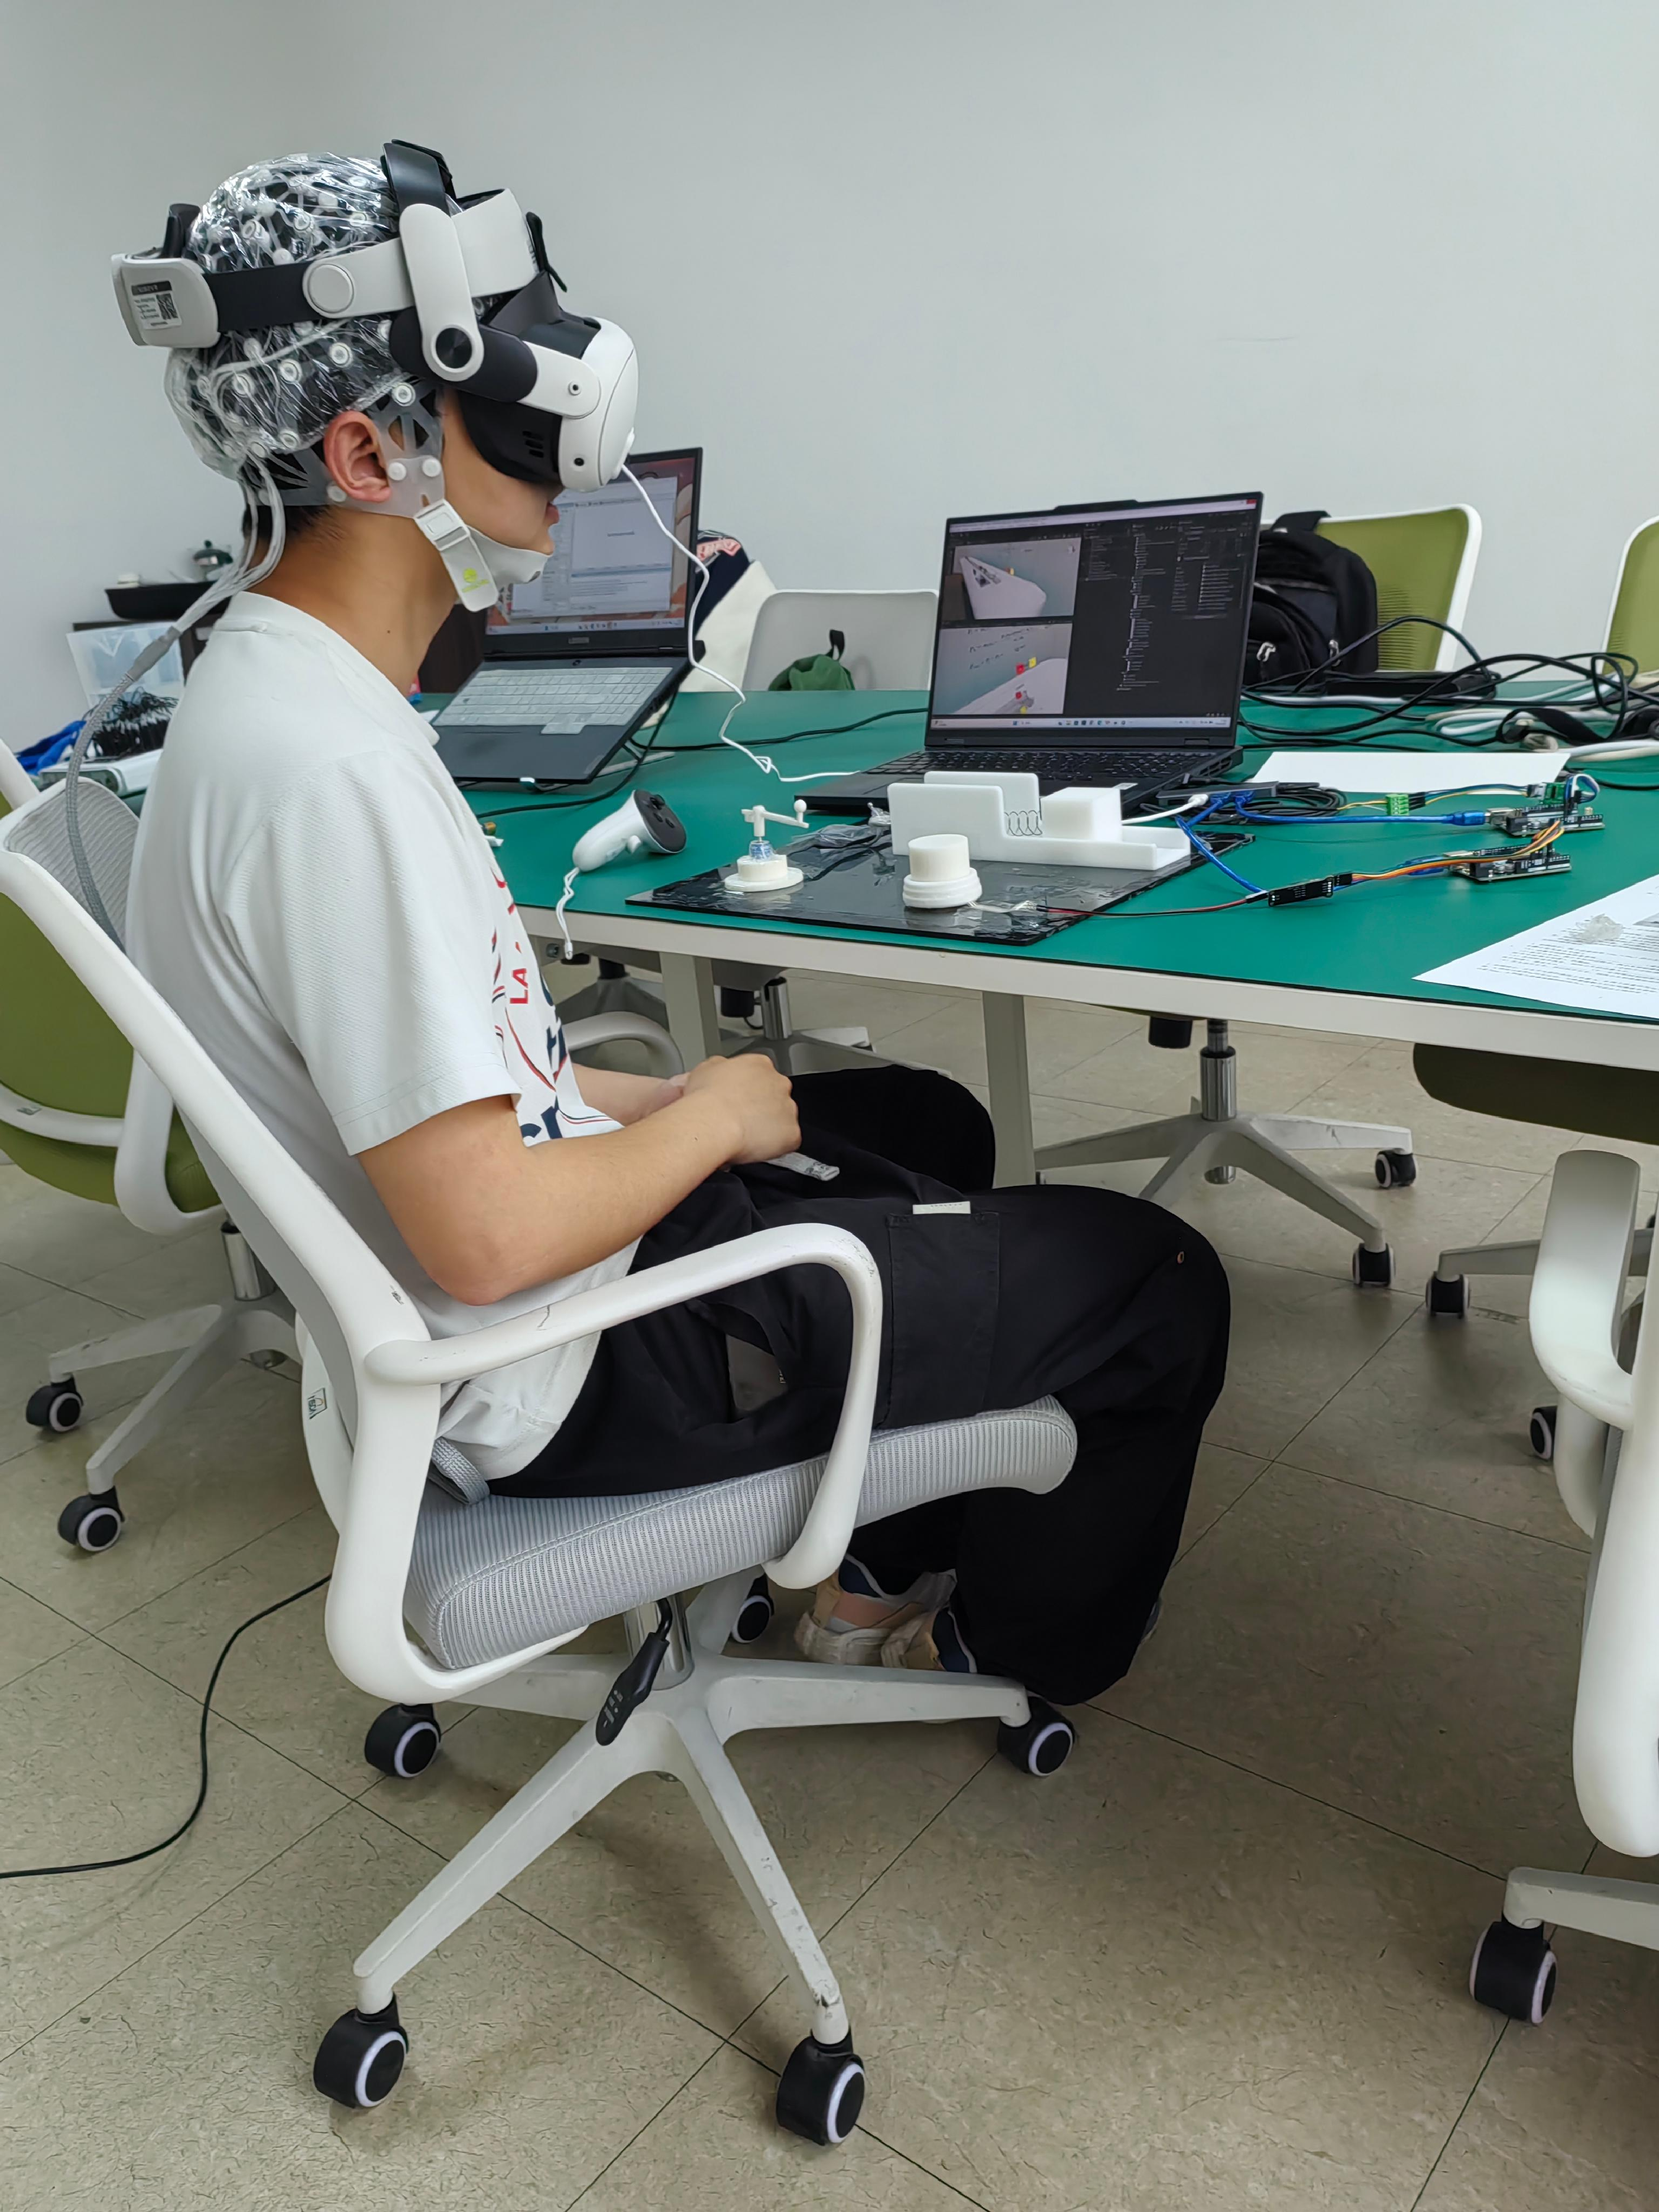
\includegraphics[width=\linewidth]{image/experiment-environment.jpg}
    \caption{评估环境}
    \label{fig:experimental-introduction}
  \end{subfigure}
  \hfill
  \begin{subfigure}{0.64\linewidth}
    \centering
    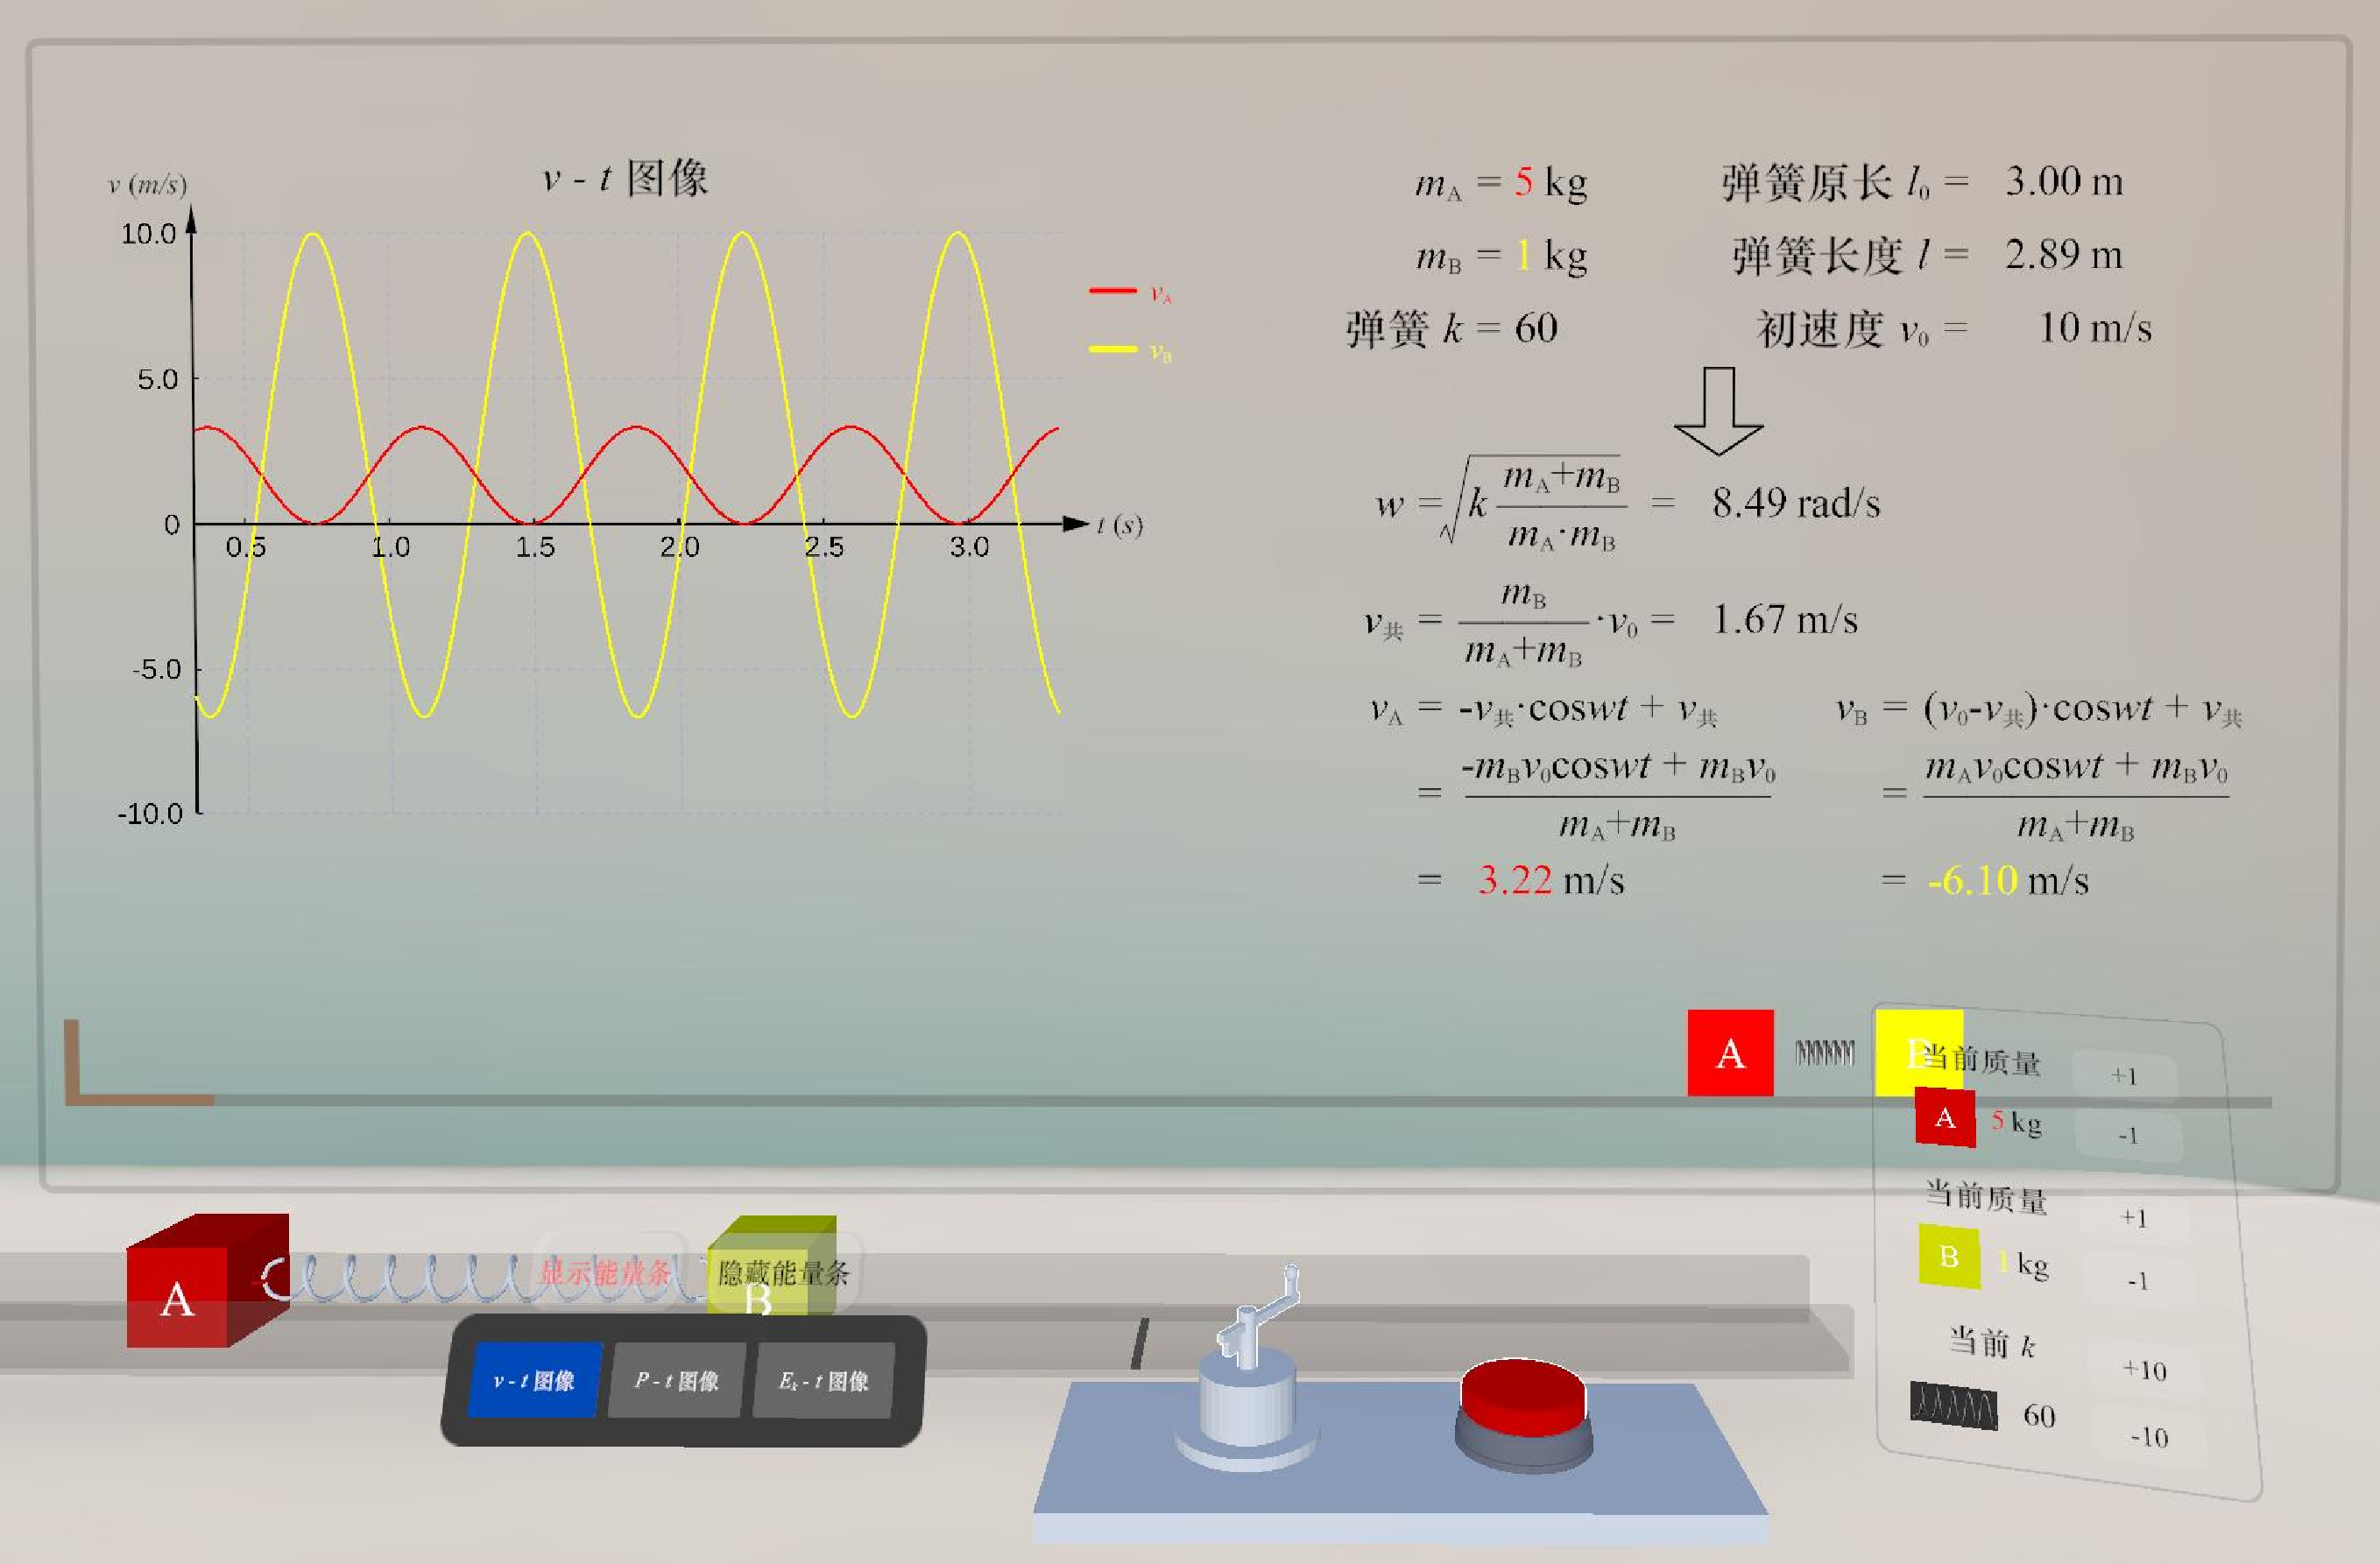
\includegraphics[width=\linewidth]{image/experiment-scenario.pdf}
    \caption{实验场景}
    \label{fig:experimental-operation}
  \end{subfigure}
  \caption{实验环境。(\subref{fig:experimental-introduction})评估实验环境,(\subref{fig:experimental-operation})实验场景}
  \label{fig:experimental-show}
\end{figure}

\begin{enumerate}[label={$\bullet$}]
  \item \texttt{硬件} Meta Quest 3 VR 头显、集成传感器的 3D 打印交互实体。
  \item \texttt{软件} 基于 Unity 2021.3 开发的虚拟实验场景,包含参数调节面板、数据可视化界面。
  \item \texttt{数据采集工具} 知识测试问卷、主观问卷量表、SynAmps2放大器(采样率1000Hz),Gelfree Net Cap盐水脑电帽。
\end{enumerate}

\subsection{实验内容与流程}
\subsubsection{实验内容}
以 “动量守恒定律验证” 为核心任务。首先,通过按钮调节物块 A、B 的质量(100-500g)和弹簧劲度系数(10-100N/m);其次,抓取拉力装置的滑块,向后拉动至指定刻度(0-10cm)后释放,观察两物块弹开过程;再次,旋转旋钮回放实验,通过虚拟面板的 v-t(速度 - 时间)、P-t(动量 - 时间)图像验证守恒规律;最后,按下按钮重置实验,记录实验数据并回答知识测试问卷。

\subsubsection{分组设计} 采用简单随机抽样分为实验组和对照组,每组 32 人。实验组(n=32) 采用手势交互,同时操作虚拟物体和 3D 打印的交互实体,获得视觉与触觉反馈;对照组(n=32)采用手势交互,通过手势操作虚拟物体,仅获得视觉反馈。

\subsubsection{实验流程}
首先,收集学生的人口统计学信息,以及先前使用VR设备和触觉反馈设备的经验,将其划分为实验组和对照组。随后,进行相关物理概念知识的前测。在正式实验之前,每个学生将练习如何使用这些设备,观看介绍整个交互任务的演示视频,仔细阅读并签署知情同意书。同时研究人员对脑电系统进行调试,并为被试佩戴脑电帽,注射导电膏,佩戴VR头显。在实验过程中,研究人员全程监督,确保被试按照实验流程进行操作,并记录实验数据。实验结束后,研究人员为每个学生发放问卷量表,并进行知识测试问卷和认知负荷量表的填写。

\subsection{测量指标}
\subsubsection{物理知识测试}
物理知识测试由 XXX 大学物理系的 XXX 教授及其团队
% 北京师范大学物理系的项华教授及其团队
提供,分为前测和后测。前后测各包含 10 项测试,每项测试记 1 分,共 10 分。前后测均选自经典高中中物理试题,涵盖动量守恒定律的基本概念、公式推导和应用。测试形式均为选择题和填空题,且所考察的知识点完全相同,仅是文字叙述方式不一致。

\subsubsection{主观问卷量表}
使用的问卷量表均为 5 分制量表。认知负荷使用Klepsch量表\cite{klepsch2017development},包括内在认知负荷、外在认知负荷和相关认知负荷三个维度;学习动机使用Keller量表\cite{keiier1987systematic},包括注意、相关、信心和满意四个维度;沉浸感使用Schubert量表\cite{schubert2001experience},包括空间存在、环境参与感和环境真实感3个维度。所有量表均经过翻译和本土化处理,确保其适用于本实验的文化和教育背景。

\subsubsection{客观生理指标}
客观生理指标为64通道脑电系统采集的Fz、Cz、Pz、Oz等关键脑区的电信号。相关研究表明,学习者认知负荷水平与脑电信号中$\alpha$波(8–13 Hz)、$\theta$波(4–8 Hz)等特定频段的能量变化存在显著的正相关关系,如表~\ref{tab:1}所示。本研究基于功率谱密度(Power Spectral Density, PSD),采用脑电领域经典的Welch方法进行PSD估计,从而揭示神经活动的状态变化。

\begin{table}
  \centering
  \setlength{\tabcolsep}{8pt} % 列间距增加(默认6pt)
  \caption{认知负荷相关实验研究}
  \begin{tabular}{cccc}
    \toprule
    研究范式 & 通道 & 频段 & 相关性                  \\
    \midrule
    N-back实验\cite{pergher2019mental} & Fz、Cz、Pz & $\alpha$、$\theta$ & 正相关\\
    字母记忆实验\cite{bashivan2015single} & 64导 & $\theta$、$\alpha$、$\beta$ & 正相关                    \\
    图片记忆实验\cite{zhang2016functional} & 16导(主要Fz) & $\theta$ & 正相关   \\
    数学运算实验\cite{so2017evaluation} & Fp1 & $\theta$ & 正相关  \\
    \bottomrule
  \end{tabular}
  \label{tab:1}
\end{table}

\section{实验结果与分析}
\subsection{物理知识测试}
使用Shapiro-Wilks检验实验组和对照组数据,结果显示均不服从正态分布,故采用Mann-Whitney U检验分析组间差异。以下数据中,显著性水平$p \le 0.05$ (*)表示显著差异,$p \le 0.01$ (**)表示高度显著差异,$p \le 0.001$ (***)表示极其显著差异。效应量解释参照Cohen准则:|r|=0.1为小效应,0.3为中效应,0.5为大效应。

\subsubsection{前测结果}
实验组和对照组在前测中没有表现出显著差异(p=0.834),因此可认为,两组的先验物理水平基本一致。

\subsubsection{后测结果}
表\ref{tab:learning-effect}展示了两组在后测中的表现,实验组的总体平均提升分值(1.156分)略高于对照组(0.656分),但未达到显著水平,效应量为中等效应。这表明触觉反馈对物理知识的整体提升存在积极趋势,但尚未形成统计学意义上的显著差异。实验组提升分值的四分位距(2 分)大于对照组(1 分),说明实验组内部学生的提升效果存在更大差异,可能与学生个体对教学干预的适应性、前期物理知识基础等因素相关。

\begin{table*}[t]
\centering
\setlength{\tabcolsep}{6pt} % 列间距增加(默认6pt)
\caption{两组前后测提升的Mann-Whitney U检验结果}
\label{tab:learning-effect}
\begin{tabular}{cccccccc}
\toprule
\textbf{维度} & \textbf{组别} & \textbf{Mean(SD)} & \textbf{Q2(Q1,Q3)} & \textbf{U} & \textbf{Z} & \textbf{p} & \textbf{|r|} \\
\midrule
\multirow{2}{*}{提升分值} 
& 实验组 & 1.156(1.749) & 1(0,2) & \multirow{2}{*}{389} & \multirow{2}{*}{-1.714} & \multirow{2}{*}{0.087} & \multirow{2}{*}{0.303} \\
& 对照组 & 0.656(1.33) & 1(0,1) \\
\bottomrule
\end{tabular}
\caption*{注:M-U检验为Mann-Whitney U检验,Q2为中位数,Q1、Q3分别为上下四分位数。}
\end{table*}

\subsection{主观问卷量表}
图\ref{fig:user-experience-result}对比两组在认知负荷、学习动机和沉浸感三个方面的差异情况。各组上方实心圆点为样本点,核平滑拟合曲线描述其分布。下方I型箱线图展示25\%(Q1)、50\%(Q2)和75\%(Q3)分位数。实验组的学习动机($Z=-3.509,p<0.001,|r|=0.620$)与沉浸感($Z=-4.751,p<0.001,|r|=0.840$)具有显著提升,为大效应。同时,实验组与对照组的总认知负荷($Z=-0.521,p=0.602,|r|=0.092$)基本一致,没有显著差异。

\begin{figure*}[t]
  \centering
  \includegraphics[width=0.75\textwidth]{image/user-experience-result.pdf}
  \caption{两组在认知负荷、学习动机和沉浸感方面的结果对比}
  \label{fig:user-experience-result}
\end{figure*}

\subsubsection{认知负荷}
两组在认知负荷方面的具体差异如表\ref{tab:cognitive-load}所示,总认知负荷无显著差异,但各子维度呈现差异化特征。从内在认知负荷来看,实验组与对照组无显著差异,这与认知负荷理论中 “内在负荷由任务本身复杂度决定” 的观点一致 —— 两组完成相同的物理实验任务,任务固有难度对认知资源的消耗相当。外在认知负荷方面,实验组得分显著低于对照组,效应量达到大效应水平。这表明触觉反馈的引入减少了虚拟环境中冗余信息的干扰,降低了不必要的认知资源消耗。相关认知负荷则呈现相反趋势:实验组显著高于对照组。这一结果说明,触觉与视觉的多感官整合促进了认知结构的建构 —— 学生通过 “拉力感受 - 弹簧形变 - 动量变化” 的联动体验,更高效地将新信息与已有物理知识(如胡克定律、动量公式)整合,形成更稳固的知识图式。因此,触觉反馈通过 “降低外在负荷、提升相关负荷” 的方式优化了认知资源分配,且未增加总体认知负担,为深度学习提供了有利条件。

\begin{table}[t]
\centering
\setlength{\tabcolsep}{2pt} % 列间距增加(默认6pt)
\caption{两组认知负荷的Mann-Whitney U检验结果}
\label{tab:cognitive-load}
\begin{tabular}{cccccccc}
\toprule
\textbf{分类} & \textbf{组别} & \textbf{Mean(SD)} & \textbf{Q2(Q1,Q3)} & \textbf{U} & \textbf{Z} & \textbf{p} & \textbf{|r|} \\
\midrule
\multirow{2}{*}{内在认知负荷} 
& 实验组 & 2.594(1.072) & 2.5(1.5,3.5) & \multirow{2}{*}{459.5} & \multirow{2}{*}{-0.720} & \multirow{2}{*}{0.472} & \multirow{2}{*}{0.127} \\
& 对照组 & 2.719(0.902) & 2.25(2,3.5) \\
% \midrule
\addlinespace
\multirow{2}{*}{外在认知负荷} 
& 实验组 & 1.479(0.301) & 1.333(1,1.917) & \multirow{2}{*}{254} & \multirow{2}{*}{-3.538} & \multirow{2}{*}{<0.001\(^{***}\)} & \multirow{2}{*}{0.625} \\
& 对照组 & 2.104(0.641) & 2(1.667,2.333) \\
% \midrule
\addlinespace
\multirow{2}{*}{相关认知负荷} 
& 实验组 & 4.208(0.622) & 4.333(4,4.667) & \multirow{2}{*}{268} & \multirow{2}{*}{-3.337} & \multirow{2}{*}{<0.001\(^{***}\)} & \multirow{2}{*}{0.590} \\
& 对照组 & 3.708(0.55) & 4(3.333,4) \\
% \midrule
\addlinespace
\multirow{2}{*}{总认知负荷} 
& 实验组 & 2.781(0.185) & 2.75(2.531,3) & \multirow{2}{*}{473.5} & \multirow{2}{*}{-0.521} & \multirow{2}{*}{0.602} & \multirow{2}{*}{0.092} \\
& 对照组 & 2.859(0.252) & 2.75(2.625,3.219) \\
\bottomrule
\end{tabular}
\end{table}

\subsubsection{学习动机}
两组在学习动机方面的具体差异如表\ref{tab:learning-motivation}所示,实验组在注意力、相关性、自信心、满意度及总学习动机上均显著高于对照组,且效应量均达到中到大效应水平。从 ARCS 动机模型视角分析:在注意力维度,实验组显著优于对照组,表明触觉反馈带来的 “操作新鲜感”(如拉动时的阻力变化)更能吸引学生持续关注实验过程;在相关性维度,实验组得分更高,因真实触感让学生更易将虚拟实验与生活经验关联,感知学习内容的实用价值;在自信心维度,实验组表现更优,这与触觉反馈降低操作难度有关 —— 学生通过物理接触确认操作有效性,减少了 “误操作焦虑”;在满意度维度,实验组优势最显著,说明成功完成实验后的 “触觉 - 视觉” 双重反馈带来了更强的成就感。

\begin{table*}[t]
\centering
\setlength{\tabcolsep}{3pt} % 列间距增加(默认6pt)
\caption{两组学习动机各维度的Mann-Whitney U检验结果}
\label{tab:learning-motivation}
\begin{tabular}{cccccccc}
\toprule
\textbf{分类} & \textbf{组别} & \textbf{Mean(SD)} & \textbf{Q2(Q1,Q3)} & \textbf{U} & \textbf{Z} & \textbf{p} & \textbf{|r|} \\
\midrule
\multirow{2}{*}{注意力} 
& 实验组 & 4.667(0.323) & 5(4.333,5) & \multirow{2}{*}{271} & \multirow{2}{*}{-3.382} & \multirow{2}{*}{0.001\(^{***}\)} & \multirow{2}{*}{0.598} \\
& 对照组 & 4.01(0.892) & 4(3.75,4.917) \\
% \midrule
\addlinespace
\multirow{2}{*}{相关性} 
& 实验组 & 4.672(0.494) & 5(4.5,5) & \multirow{2}{*}{287.5} & \multirow{2}{*}{-3.313} & \multirow{2}{*}{0.001\(^{***}\)} & \multirow{2}{*}{0.586} \\
& 对照组 & 4(1.145) & 4(3.625,5) \\
% \midrule
\addlinespace
\multirow{2}{*}{自信心} 
& 实验组 & 4.563(0.544) & 5(4,5) & \multirow{2}{*}{303.5} & \multirow{2}{*}{-3.001} & \multirow{2}{*}{0.003\(^{**}\)} & \multirow{2}{*}{0.531} \\
& 对照组 & 3.906(1.072) & 4(3.625,5) \\
% \midrule
\addlinespace
\multirow{2}{*}{满意度} 
& 实验组 & 4.573(0.167) & 4.667(4.333,5) & \multirow{2}{*}{210} & \multirow{2}{*}{-4.127} & \multirow{2}{*}{<0.001\(^{***}\)} & \multirow{2}{*}{0.730} \\
& 对照组 & 3.917(0.466) & 4(3.667,4.333) \\
% \midrule
\addlinespace
\multirow{2}{*}{学习动机} 
& 实验组 & 4.619(0.278) & 4.8(4.275,5) & \multirow{2}{*}{252.5} & \multirow{2}{*}{-3.509} & \multirow{2}{*}{<0.001\(^{***}\)} & \multirow{2}{*}{0.620} \\
& 对照组 & 3.959(0.701) & 4(3.525,4.675) \\
\bottomrule
\end{tabular}
\end{table*}

\subsubsection{沉浸感}
两组在沉浸感方面的具体差异如表\ref{tab:immersion}所示,实验组在空间存在感、投入感、真实性及总沉浸感上均显著高于对照组,且效应量普遍较大。从沉浸感理论的双维度来看:在物理 / 感官沉浸层面,空间存在感和真实性的显著差异最为突出。实验组学生因 “触摸到的拉力装置与看到的虚拟滑块同步运动”,更易产生 “身处真实实验室” 的空间错觉,而对照组仅通过视觉感知虚拟物体,难以建立稳定的空间锚点。在心理沉浸层面,投入感维度的差异表明,实验组更易进入 “深度参与” 状态。这与触觉反馈减少认知分心有关 —— 学生无需频繁校准手势,注意力可更多集中于 “观察动量变化规律” 等核心任务,从而延长专注时长。这种高沉浸感进一步强化了学习动机与认知投入的正向循环。

\begin{table*}[t]
\centering
\setlength{\tabcolsep}{2pt} % 列间距增加(默认6pt)
\caption{两组沉浸感各维度的Mann-Whitney U检验结果}
\label{tab:immersion}
\begin{tabular}{cccccccc}
\toprule
\textbf{分类} & \textbf{组别} & \textbf{Mean(SD)} & \textbf{Q2(Q1,Q3)} & \textbf{U} & \textbf{Z} & \textbf{p} & \textbf{|r|} \\
\midrule
\multirow{2}{*}{空间存在感} 
& 实验组 & 4.55(0.206) & 4.6(4.2,5) & \multirow{2}{*}{179} & \multirow{2}{*}{-4.524} & \multirow{2}{*}{<0.001\(^{***}\)} & \multirow{2}{*}{0.800} \\
& 对照组 & 3.637(0.842) & 3.8(3.2,4.2) \\
% \midrule
\addlinespace
\multirow{2}{*}{投入感} 
& 实验组 & 3.484(0.342) & 3.5(3,3.938) & \multirow{2}{*}{307.5} & \multirow{2}{*}{-2.774} & \multirow{2}{*}{0.006\(^{**}\)} & \multirow{2}{*}{0.490} \\
& 对照组 & 2.961(0.488) & 3(2.313,3.5) \\
% \midrule
\addlinespace
\multirow{2}{*}{真实性} 
& 实验组 & 3.74(0.442) & 3.667(3.333,4.333) & \multirow{2}{*}{210} & \multirow{2}{*}{-4.102} & \multirow{2}{*}{<0.001\(^{***}\)} & \multirow{2}{*}{0.725} \\
& 对照组 & 2.875(0.593) & 3(2.417,3.333) \\
% \midrule
\addlinespace
\multirow{2}{*}{沉浸感} 
& 实验组 & 3.992(0.156) & 4(3.688,4.333) & \multirow{2}{*}{159} & \multirow{2}{*}{-4.751} & \multirow{2}{*}{<0.001\(^{***}\)} & \multirow{2}{*}{0.840} \\
& 对照组 & 3.221(0.469) & 3.292(2.771,3.646) \\
\bottomrule
\end{tabular}
\end{table*}

\subsection{神经生理信号}
选取Fz、Cz、Pz、Oz电极通道,进行电信号PSD估计,最终计算得到平均功率,结果如表~\ref{tab:3}所示。

\begin{table}[t]
\centering
\setlength{\tabcolsep}{6pt} % 列间距增加(默认6pt)
\caption{不同脑区各波段平均功率比较}
\label{tab:3}
\begin{tabular}{lcccc}
\toprule
脑区(通道) & 波段 & 总体(前) & 实验组(后) & 对照组(后) \\
\midrule
\multirow{3}{*}{额叶(Fz)} & $\theta$ & 1.78 & 1.64 & 2.55 \\
 & $\alpha$ & 0.68 & 0.64 & 0.74 \\
 & $\beta$ & 0.32 & 0.17 & 0.26 \\
\addlinespace
\multirow{3}{*}{额叶中心沟(Cz)} & $\theta$ & 1.62 & 0.88 & 1.15 \\
 & $\alpha$ & 0.69 & 0.49 & 0.58 \\
 & $\beta$ & 0.26 & 0.13 & 0.19 \\
\addlinespace
\multirow{3}{*}{顶叶(Pz)} & $\theta$ & 2.02 & 1.44 & 1.53 \\
 & $\alpha$ & 1.25 & 0.97 & 0.96 \\
 & $\beta$ & 0.48 & 0.37 & 0.33 \\
\addlinespace
\multirow{3}{*}{枕叶(Oz)} & $\theta$ & 3.49 & 2.70 & 4.23 \\
 & $\alpha$ & 3.76 & 2.79 & 2.84 \\
 & $\beta$ & 2.13 & 1.85 & 1.54 \\
\bottomrule
\end{tabular}
\caption*{注:单位为$\mu V^2/\mathrm{Hz}$。}
\end{table}

由脑电信号分析可得,在Fz、Cz、Pz及Oz四个电极通道中,实验组在$\theta$、$\alpha$与$\beta$波段的平均功率均呈下降趋势,且下降幅度普遍高于对照组;相反,对照组在Fz与Oz通道的$\alpha$波平均功率出现上升。例如,Fz通道实验组后测的$\theta$波功率为1.64,显著低于对照组的2.55,且低于前测的1.78;类似地,Oz通道实验组$\theta$波功率降至2.70,而对照组升至4.23。
在脑认知研究中,额叶负责高级认知功能,如问题解决、决策制定、工作记忆、注意力调控,枕叶负责高级视觉功能,如颜色、形状、运动方向分析、视觉记忆整合\cite{kolb2009fundamentals}。结果表明,对照组学习者的大脑在执行学习任务时可能面临更大的神经资源调配压力。实验组的学生进行的触觉反馈交互有效降低了学生的认知负荷,而对照组学生进行的手势交互造成了额外的认知负荷。触觉反馈交互有助于减轻额叶区域的负荷,优化认知资源分配,从而使学生在实验过程中更轻松地学习知识,提升信息处理的效率与质量。

\section{讨论与启示}
\subsection{结果讨论}
\subsubsection{触觉反馈对知识掌握水平的影响} 
假设 H1 提出 “合适的触觉反馈能提升学习者的知识掌握水平”,实验结果显示实验组在后测中的提升分值略高于对照组(均值 1.156 vs 0.656),呈现中等效应量(|r|=0.303),但未达到统计学显著水平(p=0.087),因此认为该假设暂不成立。

这一 “积极趋势但不显著” 的结果可从三方面解释:

\begin{enumerate}[label={\arabic*)}]
  \item \texttt{短期干预的局限性} 实验任务聚焦 “动量守恒定律验证” 单一知识点,单次干预时长有限。触觉反馈对知识的深层内化可能需要更长周期 —— 多感官整合形成的神经通路需反复强化才能转化为稳定的知识表征。后续研究可延长干预周期,观察长期学习效果。
  \item \texttt{知识测量的敏感性} 当前测试以选择题和填空题为主,侧重知识的再认与回忆。而触觉反馈的优势可能体现在概念的直观化建构(如 “力的作用与动量变化的关联”),这类深层理解需通过开放性问题或操作任务进一步测量。
  \item \texttt{个体差异的调节作用} 实验组提升分值的四分位距(2 分)大于对照组(1 分),提示触觉反馈的效果可能受学习者空间认知能力、动手操作经验等个体特质影响。后续可通过回归分析挖掘调节变量,为个性化反馈设计提供依据。
\end{enumerate}

尽管未达显著水平,中等效应量仍表明触觉反馈对知识学习存在积极影响,需扩大样本量进一步验证。

\subsubsection{触觉反馈对交互体验的优化机制}
假设 H2 提出 “合适的触觉反馈能改善学习者的交互体验”,实验结果对此提供了强有力支持:实验组在学习动机和沉浸感上均表现出显著提升,且认知负荷结构更优。因此,我们认为该假设成立,其内在机制分析如下:

\begin{enumerate}[label={\arabic*)}]
  \item \texttt{认知负荷的结构性优化} 实验组外在认知负荷显著降低,而相关认知负荷显著提高,且总负荷不变。这一结果契合认知负荷理论 —— 触觉反馈通过认知消耗降低外在负荷,同时通过促进多表征整合提升相关负荷,最终实现认知资源的高效分配。
  \item \texttt{学习动机的 ARCS 模型解析} 注意力方面,触觉反馈的 “新奇性” 通过外周神经刺激持续激活注意网络,避免单一视觉输入导致的疲劳;相关性方面,真实触感使抽象物理量(如劲度系数)与生活经验(如拉橡皮筋的手感)建立联结,提升知识的 “有用性感知”;自信心方面,触觉反馈降低了虚拟操作的 “不确定性”(如确认滑块已拉至指定刻度),减少操作焦虑;满意度方面,“触觉 - 视觉” 双重反馈强化了操作的 “闭环感”,使实验成功的成就感更强烈。
  \item \texttt{沉浸感的多维度增强} 实验组在空间存在感和环境真实性上的大效应量,印证了 “触觉是建立虚拟环境真实感的核心线索” 这一观点。3D 打印实体与虚拟物体的运动同步性(拉动滑块时的阻力反馈)为学习者提供了稳定的 “感官锚点”,减少了视觉独有的 “悬浮感”,从而强化 “身处真实实验室” 的空间错觉。
\end{enumerate}

\subsection{教育启示}
\subsubsection{对虚拟实验教学设计的启示}
触觉反馈需遵循 “适度性” 原则,并非反馈强度越高效果越好,需根据知识点特性设计 “恰到好处” 的触觉线索。例如,动量守恒实验中,拉力装置的阻力反馈应与虚拟弹簧的劲度系数严格匹配,避免过度反馈干扰物理规律的感知。此外,针对实验组内部提升差异较大的现象,可设计自适应反馈系统。对操作困难的学习者,增加触觉引导以降低外在负荷;对能力较强的学习者,提供可变参数的触觉挑战以提升相关负荷。

\subsubsection{对中学物理教学实践的启示}
首先,动量、力等物理量的抽象性是教学难点,借助触觉反馈,可将 “动量变化” 转化为 “手部受力的冲量感”,将 “劲度系数” 转化为 “拉动时的阻力差异”,帮助学生建立 “具身认知”。其次,传统的物理实验受限于设备成本或安全性,而 VR + 触觉反馈可模拟危险场景,让学生在安全环境中获得 “沉浸式操作” 经验。最后,实验组在满意度维度的高效应量提示,触觉反馈带来的 “愉悦感” 可转化为持续学习的动力。教师可将此类虚拟实验作为课前预习或课后拓展工具,弥补传统课堂的互动局限性。

\subsubsection{对教育技术发展的启示}
首先,当前 3D 打印交互实体仍存在定制成本高、便携性不足的问题。未来可研发模块化触觉设备,降低学校应用门槛。其次,本研究未深入分析了神经生理信号,后续可探索触觉反馈对大脑激活模式的影响,为神经教育学的设计提供依据。最后,物理实验中的触觉反馈设计需融合物理学、心理学等多学科知识,未来可建立 “教育技术 - 学科教学 - 工程设计” 的协同研发机制。

\section{结语}
本研究以高中物理 “动量守恒定律验证” 实验为载体,系统探究了沉浸式手势学习环境中触觉反馈对物理学习效果的影响,通过整合物理知识测试、主观问卷量表及客观生理指标的多模态数据分析,系统探究了触觉反馈对交互体验与知识掌握的差异化影响。研究结果表明,在虚拟实验场景中引入触觉反馈,虽未对学习者的知识掌握水平产生统计学意义上的显著提升(p=0.087),但呈现出中等效应的积极趋势;同时,其能显著增强学习者的学习动机(p<0.001)与沉浸感(p<0.001),并通过降低外在认知负荷、提升相关认知负荷实现认知资源的结构性优化,且未增加总体认知负担(p=0.602)。这些发现为理解多感官交互在沉浸式学习中的价值提供了实证依据,也为教育技术与学科教学的融合创新开辟了新视角。

未来研究可拓展至更多学科内容(如力学、电磁学)并延长干预周期,以验证触觉反馈的长期影响与跨学科适用性。同时,本次研究知识测试以再认与回忆类题目为主,后续可增加开放性问题、问题解决任务等,更精准地评估深层理解能力。

\begin{credits}
\subsubsection{\ackname} 
本研究得到国家自然科学基金 XXX 
% (编号62377004)
支持。

\subsubsection{\discintname}
作者声明无利益冲突。
\end{credits}

\bibliography{VRTI-bib}

\end{document}